\documentclass{scrartcl}
\usepackage[utf8]{inputenc} 
\usepackage[T1]{fontenc}
\usepackage{lmodern}
\usepackage[ngerman]{babel}
\usepackage{courier}
\usepackage{amsmath}
\usepackage{graphicx}
\usepackage{multicol}
\usepackage{geometry}
\usepackage{authblk}
\usepackage[font=scriptsize, labelfont=bf]{caption}
\newenvironment{Figure}
  {\par\medskip\noindent\minipage{\linewidth}}
  {\endminipage\par\medskip}


% for skript letters like H...
\usepackage{mathrsfs}

\geometry{verbose,a4paper,tmargin=25mm,bmargin=25mm,lmargin=15mm,rmargin=20mm}

\title{Protokoll zum Versuch Nichtlineare Dynamik und Chaos}
\author{Nicolas Heimann, Jesse Hinrichsen}
\affil{\textit{Universität Hamburg}}
\date{2015}
\begin{document}
\maketitle




\begin{description}
\item Zusammenfassung
\end{description}


\section{  Einleitung  }
LALALA

\section{Logistische Abbildung}
$$x_{n+1}=f_r(x_n)=rx_n(1-x_n)$$
Def.: $f^2(x) = f(f(x))$
$$\Rightarrow x_{n+2}=r^2x_n(1-x_n)(1-rx_n(1-x_n))$$
\newline
Fixpunktgleichung (Einerzyklus): 
$$x=rx(1-x)$$
$$\Rightarrow x_1=0, x_2=1-\frac{1}{r}$$
Startwerte x=0 und x=1 haben den Fixpunkt $x_1$ wohingegen für alle $x\in (0,1)$ der Fixpunkt $x_2$ ist.
\newline
Fixpunktgleichung (Zweierzyklus):
$$x=r^2x(1-x)(1-rx(1-x))$$
$$\Rightarrow x_{3,4}=\pm\frac{\sqrt{r^2-2 r-3}+r+1}{2 r}$$
Damit $x_{3,4}$ reel bleibt muss $r^2-2 r-3 \geq 0$
$$\Rightarrow r \leq -1 \land r \geq 3$$
Für diesen Bereich gibt es folglich 2 weitere Fixpunkte $x_{3,4} \Leftrightarrow$ Perdiodenverdopplung 
\newline
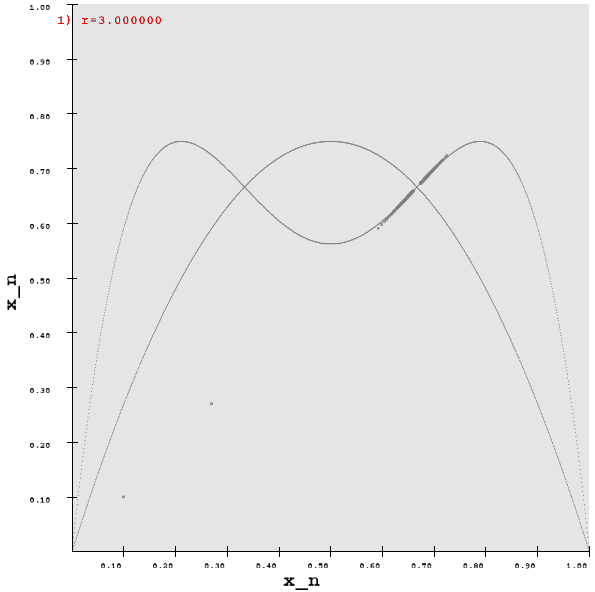
\includegraphics[scale=0.3]{r3}
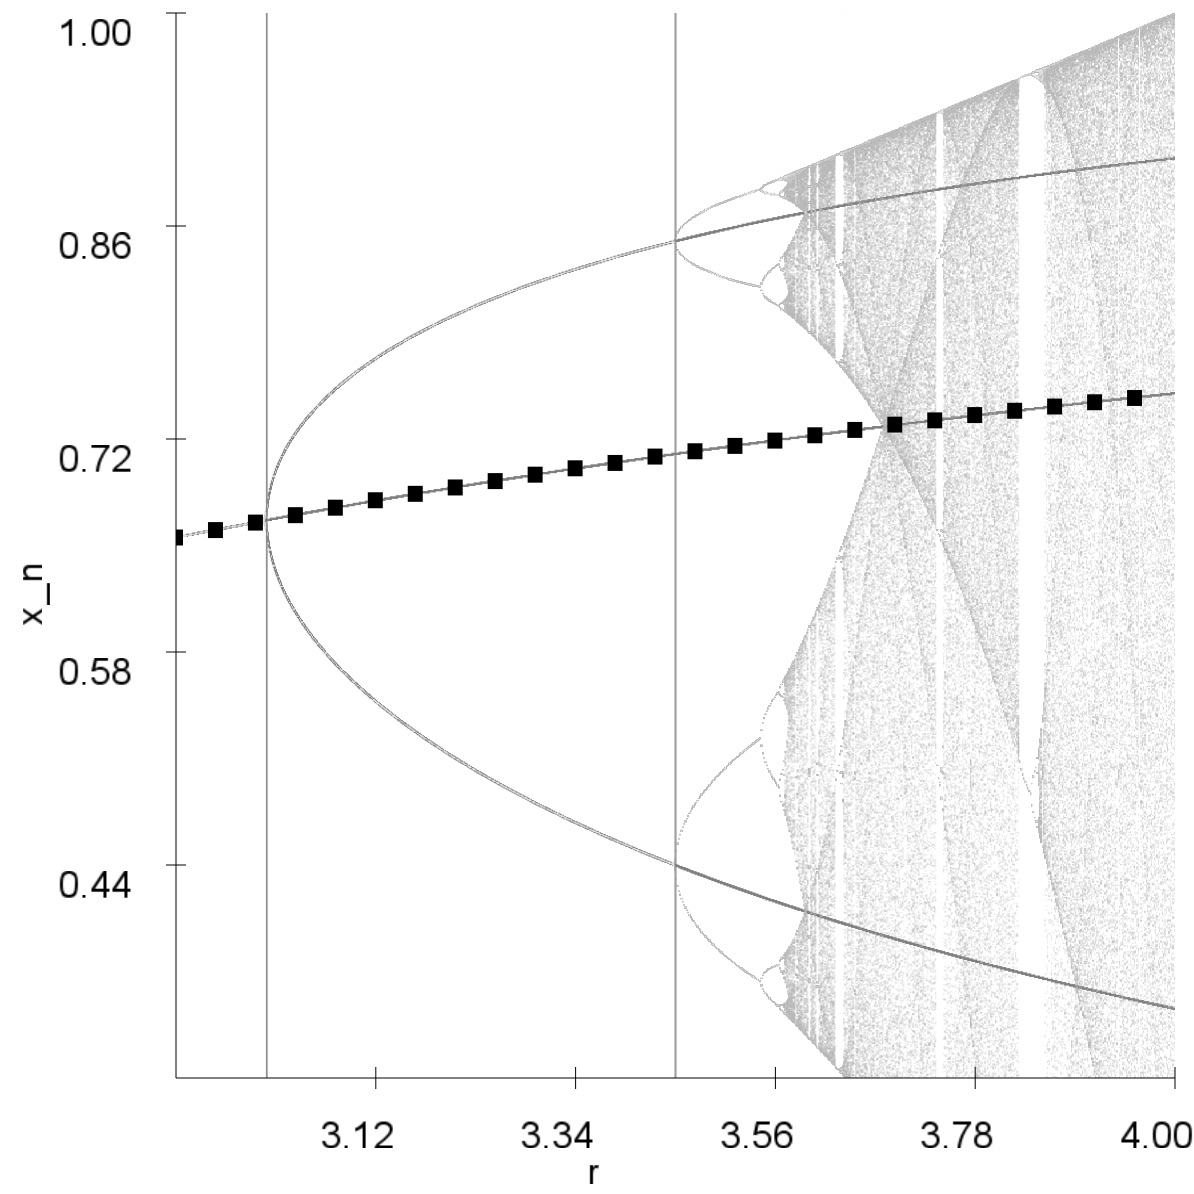
\includegraphics[scale=0.3]{analy-periodenv}
Stabilitätsbedingung:
$$\mid f'(x)\mid <1, mit f'(x)=r(1-x) folgt$$
$$\mid r(1-x)\mid < 1$$
$$\Leftrightarrow \mid 1-x\mid < \mid \frac{1}{r}\mid$$

\section{ Literatur }
\begin{itemize} 
\item Nichtlineare Dynamik und Chaos - Physikalisches Praktikum für Fortgeschrittene Universität Hamburg
\end{itemize}




\end{document}







